\chapter{Algorithm}
\newpage
\begin{center}
  \captionof{figure}{A flowchart detailing a single iteration of the algorithm.}
  % setting the typeface to sans serif and the font size to small
  % the scope local to the environment
  \sffamily
  \footnotesize
  \begin{tikzpicture}[auto,
    %decision/.style={diamond, draw=black, thick, fill=white,
    %text width=8em, text badly centered,
    %inner sep=1pt, font=\sffamily\small},
    block_center/.style ={rectangle, draw=black, thick, fill=white,
                          text width=8em, text centered, minimum height=4em},
    block_left/.style ={rectangle, draw=black, thick, fill=white,
                        text width=16em, text ragged, minimum height=4em, inner sep=6pt},
    block_noborder/.style ={rectangle, draw=none, thick, fill=none,
                            text width=22em, text centered, minimum height=1em},
    block_assign/.style ={rectangle, draw=black, thick, fill=white,
                          text width=18em, text ragged, minimum height=3em, inner sep=6pt},
    block_lost/.style ={rectangle, draw=black, thick, fill=white,
                        text width=16em, text ragged, minimum height=3em, inner sep=6pt},
    line/.style ={draw, thick, -latex', shorten >=0pt}]
    % outlining the flowchart using the PGF/TikZ matrix funtion
    \matrix [column sep=-10mm,row sep=3mm] {
        \node [block_noborder] (e) {}; \\
        % Lidar Scan
        \node [block_center] (lidarScan) {Lidar Scan}; \\
        % 150,000 points 
        \node [block_noborder] (150p) {$\sim$ $150,000$ points}; \\
        % Remove Static Map
        \node [block_center] (staticMap) {Static Map Removal}; \\
        % 30,000 points
        \node [block_noborder] (30p) {$\sim$ $20,000$ points}; \\
        % Clustering 
        \node [block_center] (clustering) {Clustering}; \\
        % Potential dynamic objects 
        \node [block_noborder] (potential) {$\sim$ $10,000$ points\\ $20$-$30$ clusters: Potential dynamic objects}; \\
        % Neural Network
        \node [block_center] (nn) {Neural Network}; \\
        % Tagged Objects 
        \node [block_noborder] (ped) {Pedestrians, crowds, cyclists, unknown targets}; 
            &
            \node [block_noborder] (cars) {cars}; \\
        % Ellip PHD & Car pre-processing
        \node [block_center] (ellip) {Elliptical PHD filter};
            &
            \node [block_center] (pre) {Car Cluster Pre-processing}; \\
        % Estimated shape & state Corner Point   
        \node [block_noborder] (e) {}; \\
        \node [block_noborder] (ellipState) {Elliptical shape, size \& state estimation};
            & 
            \node [block_noborder] (cp) {Viewed width \& length, corner point}; \\
        % Car PHD
            &
            \node [block_center] (rect) {Rectangular PHD filter}; \\
        \node [block_noborder] (e) {};
            &
            \node [block_noborder] (rectState) {Rectangular shape, size \& state estimation}; \\
        % Estimated Targets 
        \node [block_center] (targets) {Targets}; \\
    };% end matrix
    % connecting nodes with paths
    \begin{scope}[every path/.style=line]
      % paths for enrollemnt rows
      %\path (referred)   -- (excluded1);
        \path (lidarScan)   -- (150p);
        \path (150p)        -- (staticMap);
        \path (staticMap)   -- (30p);
        \path (30p)         -- (clustering);
        \path (clustering)  -- (potential);
        \path (potential)   -- (nn);
        \path (nn)          -- (ped);
        % Left 
        \path (ped)         -- (ellip);
        \path (ellip)       -- (ellipState);
        \path (ellipState)  -- (targets);
        % Right 
        \path (nn)          -| (cars);
        \path (cars)        -- (pre);
        \path (pre)         -- (cp);
        \path (cp)          -- (rect);
        \path (rect)        -- (rectState);
        \path (rectState)   |- (targets);
    \end{scope}
  \end{tikzpicture}
\end{center}

\section{Sensor Properties}

\begin{figure}
    \centering
    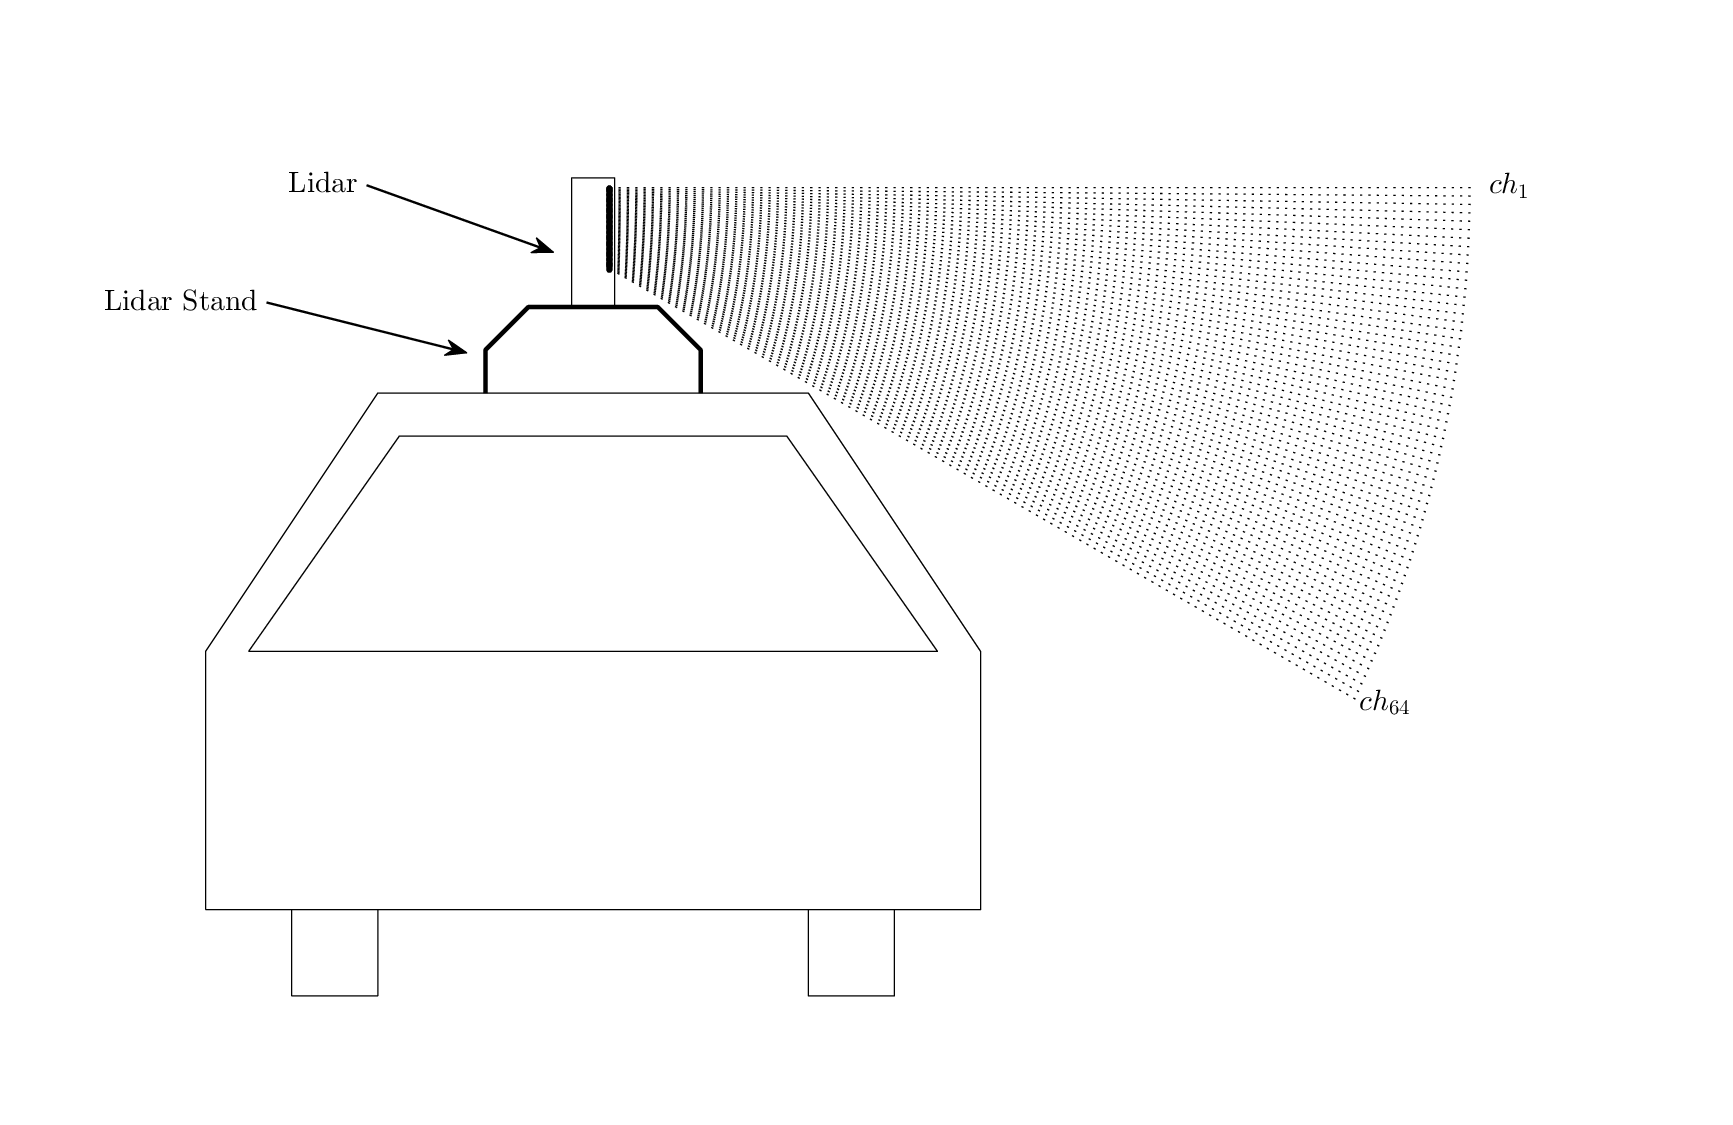
\includegraphics[width= \linewidth]{include/images/lidarImg.png}
    \caption{Caption}
    \label{fig:my_label}
\end{figure}
\todo{image of the 64 laser beams towards the ground to explain why objects have fewer and fewer points the further away they are, why there are so many ground points, write about sensor frequency and so on}

\section{Static Point Removal}

\subsection{Ground Removal}
In a typical traffic environment, LIDAR data captured by a sensor mounted on the roof of a vehicle contains a substantial amount of points that simply describe the ground. Those usually amount to around 50-70\% of the points in one frame. In this thesis those ground points are not useful for any practical purpose and are therefore removed.

The employed algorithm lays a grid over the point cloud in the x-y-plane. For every grid cell the points, whose z-value falls within the lower $c$\% of the entire cell, are removed. Figure \ref{fig:ground_removal} shows the difference between an unprocessed lidar frame and the same frame after the ground removal algorithm.

\begin{figure}[H]
\centering
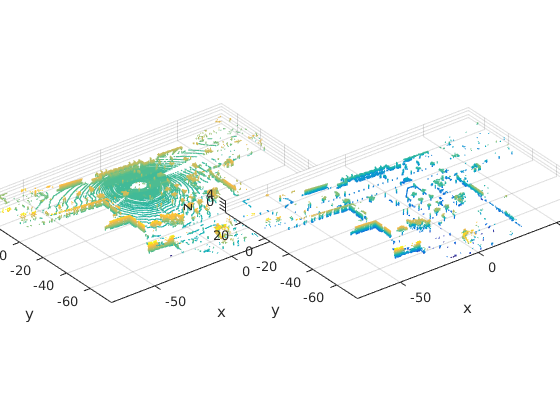
\includegraphics[width = \textwidth]{include/images/ground_remove.png}
\caption{an unprocessed frame (left) and the same frame with the ground points removed (right)}
\label{fig:ground_removal}
\end{figure}

\begin{algorithm}[H]
\caption{Remove Ground Points}\label{ground_point}
\begin{algorithmic}
\Input Set of points $P$, number of grid columns/rows $n$, cut-off $c$
\Init $P_{keep} \leftarrow \emptyset$ as the set of points to keep   
\For{$i=1$ to $n$} 
\For{$j=1$ to $n$}
\State $P_{ij} \leftarrow$ get all points that lie within cell $ij$
\State $z_{ij,max}, z_{ij,min} \leftarrow$ calculate max and min z value for points $P_{ij}$
\State $P_{ij,keep} \leftarrow$ keep only the points that have a z value above $c (z_{ij,max} - z_{ij,min})$
\State $P_{keep} \leftarrow (P_{keep} \cup P_{ij,keep})$  
\EndFor
\EndFor
\Output $P \leftarrow P_{keep}$, set of points that are not ground points
\end{algorithmic}
\end{algorithm}

The cut-off percentage $c$ and the number of grid columns/rows $n$ are design parameters that influence the performance of the algorithm. A higher cut-off will remove the ground points more robustly but might impact the quality of the processed data by e.g. "cutting off" tyres of cars or lower legs of pedestrians. More grid cells will allow for a more fine-tuned result by making it less likely that big and small objects end up in the same cell which usually results in removing substantial parts of the smaller object. However, the smaller the cell size, the longer the computation time of the algorithm.

In this thesis values of $n=200$ and a cut-off of $c=0.3$ were found to be a good compromise between performance and speed. The algorithm removes about $80,000$ to $110,000$ points which is a great reminder of the huge amount of data that lidar sensors produce and the emphasis on pre-processing that is needed to be able to use that high resolution practically.

\subsection{Static Objects}
A core part of this thesis was to determine the eligibility of using a priori information about the environment in order to easily dismiss static parts of the data. The high resolution of a lidar sensor is very useful for gathering detailed information about surrounding targets. Unfortunately this also means that the raw data contains a lot of information about objects that are not useful for the purpose of this thesis. Being able to dismiss static data in a straightforward way could therefore greatly ease the computational load of all following steps of the algorithm.

The static map is made up of simple cuboids that describe walls, buildings and trees. Figure \ref{fig:static_map_campus} shows an example of such a map in comparison with the point cloud data captured by the sensor. \todo{should we describe that we made the static map ourselves based on seeing that it actually worked with Annie's map, which we then couldn't use because ÅF didn't manage to get some suitable data in 4 months?}

\begin{figure}[H]
\centering
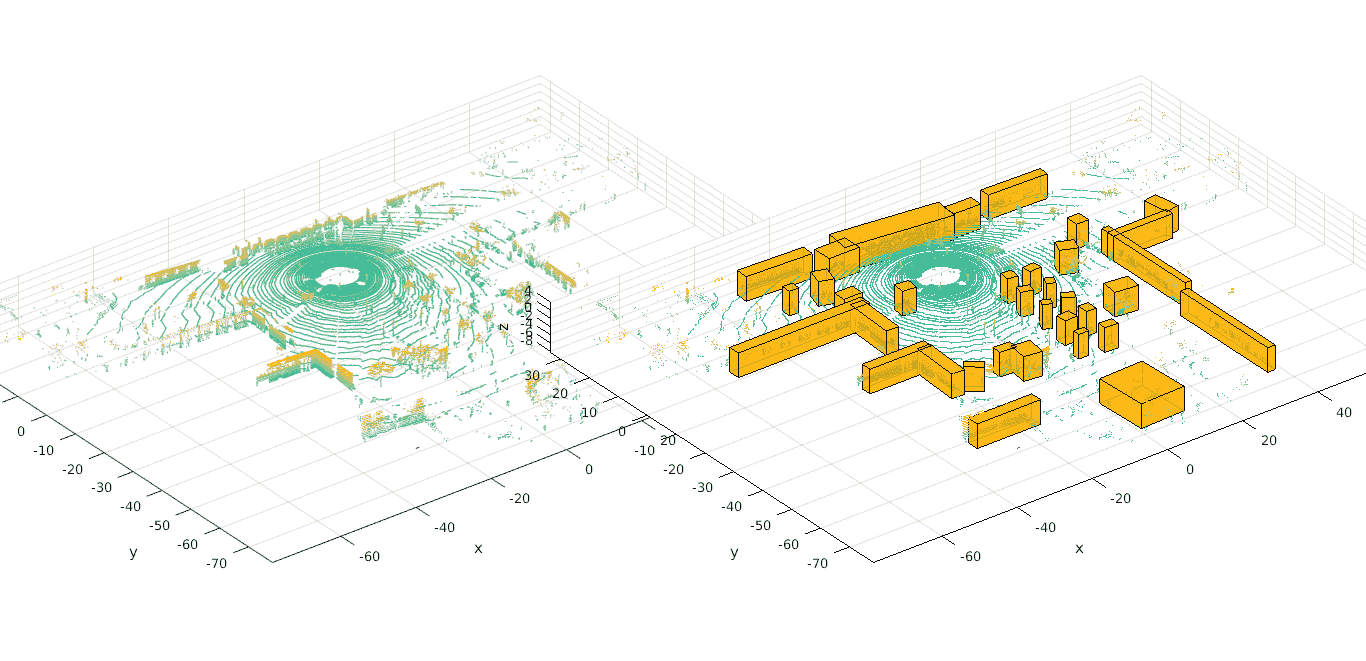
\includegraphics[width = \textwidth]{include/images/static_map_campus.png}
\caption{lidar data (left) and the same data overlain by the static map (right)\protect\footnotemark}
\label{fig:static_map_campus}
\end{figure}

\footnotetext{N.B. the ground points seen in both images would usually have been removed at this stage of the algorithm but were left in this Figure to make it easier to see where the static map cuboids are positioned within the frame}

Since all corner points $p_{cor}$ and the center of each cuboid $p_{cen}$ are known, a simple geometrical approach was chosen. First, the normal vector for each of the 6 faces is calculated. Those vectors are then used to determine whether $p_{cen}$ has a positive or negative distance to each of the faces. Now by checking whether the point to test $p_{test}$ has the same type of distance (negative or positive) towards each face it can be determined whether $p_{test}$ lies within the cuboid or not. The following pseudocode describes the entire process as a nested loop over all points and all cuboids.

In practice it was also found that the algorithm can be sped up significantly by first ordering the set of all cuboids by distance from the current ego position. Since a lidar sensor captures fewer and fewer points the further away an object is, it is reasonable to test against the cuboids in order of increasing distance from the sensor. Any point that is removed at an early stage in the algorithm will not have to be checked against all the other cuboids anymore.

\begin{algorithm}[H]
\caption{Remove Static Points}\label{static_point}
\begin{algorithmic}
\Input Set of points $P$, Set of cuboids $C$
\Init Sort $C$ by distance to current ego position (ascending)
\For{$j=1$ to $C$} 
\State calculate normal vectors for each of the 6 faces of $C_j$ 
\State $\vec{d}_j \leftarrow$ calculate the distance vector of the center $c_j$
\EndFor
\For{$i=1$ to $P$} 
\For{$j=1$ to $C$} 
\State $\vec{d}_{ij} \leftarrow$ calculate the distance vector of $p_i$
\If{$\vec{d}_{ij}./abs(\vec{d}_{ij}) - \vec{d}_{j}./abs(\vec{d}_{j}) = \vec{0}$}
\State remove $p_i$ from $P$
\State \textbf{break}
\EndIf
\EndFor
\EndFor
\Output Set of points $P$ that are not within any of the cuboids
\end{algorithmic}
\end{algorithm}

The algorithm effectively reduces the data by about $20,000$ to $30,000$ points and is a key ingredient to speed up the subsequent clustering and filtering.

\section{Clustering}

At this point the pointcloud usually contains somewhere between $10,000$ and $20,000$ points and looks like the example in Figure \ref{fig:cloud_before_clustering}. 

\begin{figure}[H]
\centering
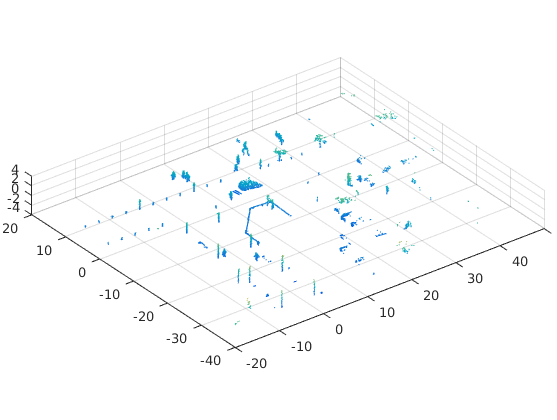
\includegraphics[width = .9\textwidth]{include/images/cloud_before_clustering.png}
\caption{a typical pointcloud frame after removing the ground and static objects}
\label{fig:cloud_before_clustering}
\end{figure}

As you can see, distinct objects start to show up in the data very clearly. However, the data is still only a set of points with no indication of whether a pair of points might belong to the same object or not. Clustering uses the fact that measurements originating from the same object are assumed to be spatially very close.

What kind of clusters are found can be steered by two parameters: the minimum number of points in a cluster $n_{min}$ and the maximum distance between any two points in a cluster that are closest to each other $d_{max}$. 

The implemented algorithm builds on creating a k-d-tree structure of the points to be clustered. k-d-trees allow for efficient nearest-neighbour searches (nnsearch) that are important for this application. A k-d-tree is built by continually branching the tree over hyperplanes that divide the entire space into smaller and smaller subspaces. Each point is a node of the tree, with points that are on the same side of any of the dividing hyperplanes ending up in the same branch of the tree. For a very accessible introduction to k-d-trees the reader is referred to \cite{Moore_1991_2818_kd}.

\begin{algorithm}[H]
\caption{Clustering Points}\label{cluster_point}
\begin{algorithmic}
\Input Set of points $P$, $m_{min}$, $d_{max}$
\Init build a k-d-tree from $P$, empty set of clusters $C$
\State $i = 0$
\While{$P \neq \emptyset$}
\State $C_i = \emptyset$, initialize a new empty cluster
\State $T \leftarrow P_0$, initialize a new temporary set with the current first point in $P$ 
\While{$T \neq \emptyset$}
    \State $X \leftarrow \text{nnsearch}(T_0, d_{max})$, find all neighbors with less than $d_{max}$ distance to $T_0$
    \State $T \leftarrow T \cup X$, add all the points $X$ to $T$
    \State $C_i \leftarrow C_i \cup T_0$
    \State $T \leftarrow T\setminus T_0$
\EndWhile
\If {$|C_i| \geq m_{min}$}
    \State $C \leftarrow C \cup C_i$, add the new cluster to the set of clusters
    \State $P \leftarrow P \setminus C_i$
    \State $i \leftarrow i+1$
\Else
    \State $P \leftarrow P \setminus C_i$
    \State $C_i \leftarrow \emptyset$
\EndIf
\EndWhile
\Output Set of clusters $C$
\end{algorithmic}
\end{algorithm}

In this thesis it was found that values of $n_{min} = 50$ and $d_{max} = 0.7m$ delivered good results. Having a fixed threshold is certainly not optimal when using a range sensor like lidar whose data resolution decreases proportional to the distance from the sensor. A pedestrian that might be defined by $\approx 200$ points when $10m$ away from the sensor, may only end up being composed of $\approx 20$ points at $100m$ distance. However, the mentioned values were found to be very robust for all objects of interest within a radius of $50m$ around the sensor.

Considering Figure \ref{fig:cloud_before_clustering} the goal with clustering is quite diverse. Ideally one would like distinct objects to also be clustered as distinct clusters. This can be quite a challenging task sometimes, e.g. for two pedestrians that walk very close to each other. One would also like to dismiss tiny objects like tree branches or fence poles that survived the static point removal and are known to be much smaller than any object this thesis is potentially interested in (i.e. smaller than a pedestrian). 

\begin{figure}[H]
\centering
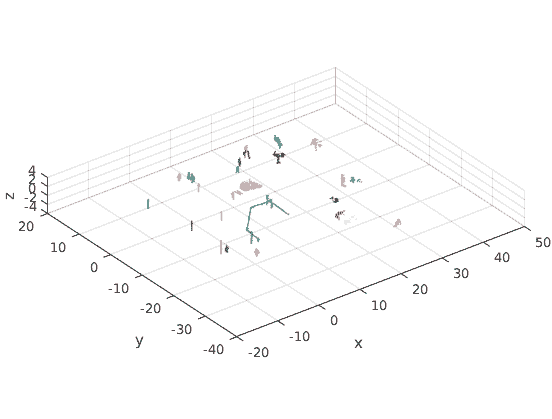
\includegraphics[width = .9\textwidth]{include/images/cloud_after_clustering.png}
\caption{a typical pointcloud frame after clustering, different colors indicate different clusters}
\label{fig:cloud_after_clustering}
\end{figure}

Figure \ref{fig:cloud_after_clustering} shows the result of the clustering step performed on the frame in Figure \ref{fig:cloud_before_clustering}. It can be seen that a lot of tiny objects could be dismissed and all other major objects are successfully clustered. However, some typical clustering problems can be observed as illustrated in Figure \ref{fig:clustering_problems}.

\begin{figure}[H]
\centering
\begin{subfigure}{.5\textwidth}
  \centering
  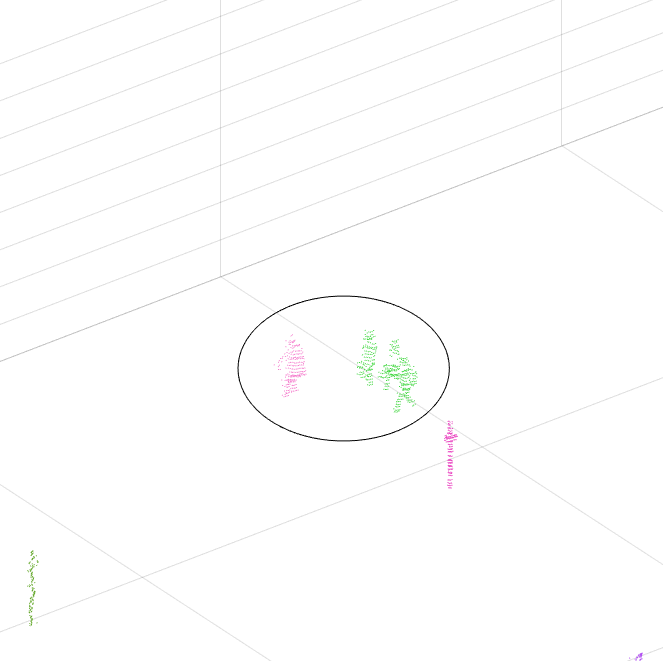
\includegraphics[width=1.0\linewidth]{include/images/clustering_problems_1.png}
\end{subfigure}%
\begin{subfigure}{.5\textwidth}
  \centering
  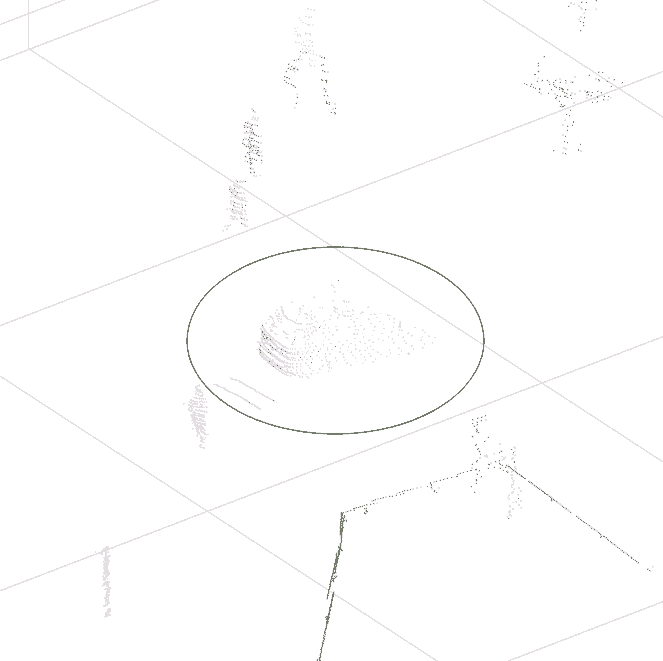
\includegraphics[width=1.0\linewidth]{include/images/clustering_problems_2.png}
\end{subfigure}
\caption{two common clustering problems: a group of 4 pedestrians, 3 of which get clustered into the same cluster (left) and a car that is being clustered together with some nearby ground points (right)}
\label{fig:clustering_problems}
\end{figure}

\todo{write about what could be done about those problems and why we chose not do that?}

\section{Classification}

The performance of the object-tracking filter based on lidar data can be greatly enhanced by using knowledge about the different objects that will be encountered in typical traffic scenarios. At this point, the pre-processing steps have broken down the vast amount of initial points to a small number (usually 10-20) of clusters.

The subsequent filter's task is now to both track all dynamic objects and reject clutter. It is hugely beneficial to the filter's performance to know whether a cluster is an object of interest or clutter (like fragments of walls, trees or poles that survived the pre-processing). The scope of this thesis limits the former to pedestrians, cyclists and cars.

The question is whether the shape of the clusters can be used to determine what type of object it is. This is a typical classification problem, which can be solved with a Machine Learning approach. From looking at lidar data, e.g. Figure \ref{fig:clustering_problems}, it becomes clear that it captures the environment with a clear perception of both depth and shapes. It is easy to detect not only cyclists and cars but also pedestrians with the naked eye, which is usually a promising indicator that such a task can indeed be solved by Machine Learning. 

Therefore it indeed seemed promising to try and classify objects that are within a reasonable range of the sensor. This was found to be about $50m$, after that the resolution of objects starts to decrease quite rapidly. The classification also seems like a reasonable idea to pursue in the sense that a Bayesian framework always tries to include every possible prior information available. 

Finally a data-driven algorithm for object classification made sense from a runtime point of view. The initial training might be time-intensive, but the eventual hypothesis function will be a simple mapping from certain features of a cluster (such as height, length, width or center point) to a classification vector. This function will therefore scale linearly with the number of clusters to classify and will be much faster than any other part of the pipeline. The expected increase in performance is therefore a good bargain.

\subsection{Features}

At the heart of any Machine Learning algorithm lie the features that are used to quantify each of the available datapoints. In this thesis, those datapoints are the individual lidar clusters. The aim is to choose those features in a way that they have very distinct values for the respective classes that you expect to appear in the data. Initial guesses for potential features can often be derived from human intuition. Figure \ref{fig:features_intuition} shows examples of typical lidar representations of the three objects of interest while being approximately equidistant to the sensor position.

\begin{figure}[H]
\centering
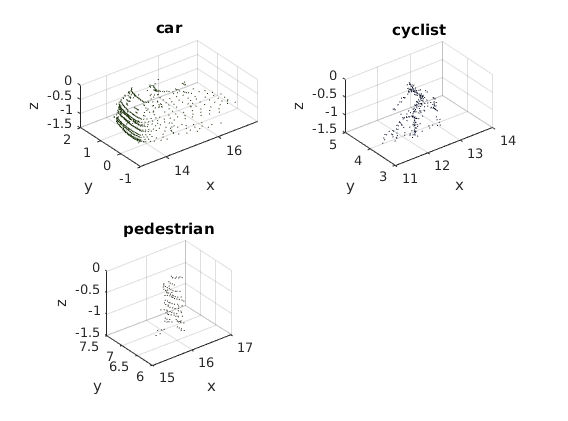
\includegraphics[width = \textwidth]{include/images/features_intuition.png}
\caption{typical lidar representations of the three objects of interest}
\label{fig:features_intuition}
\end{figure}

As you can see, there are obvious differences in the dimensions of all three objects especially in $x$ and $y$ direction. Therefore the width $w$, length $l$ and height $h$ of the clusters were considered to be valuable features.  Also, while the pedestrian has all it's points spread quite closely around the center, the points of a car or cyclist are more widespread. Thus the point density $\rho$ was viewed as a valuable feature. In addition to that, although not directly visible in Figure \ref{fig:features_intuition}, the total number of points $n$ is different in all three objects. The car consists of $\approx 800$, the cyclist of $\approx 200$ and the pedestrian of $\approx 100$ points, which shows that the number of points contains a lot of informative value. However, since the number of points of an object decrease for an increasing distance to the sensor, the number of points was divided by the distance $d$ of that cluster towards the sensor.

The final feature vector was therefore:

\begin{equation}
     f = [w\quad l\quad h\quad \rho\quad \frac{n}{d}]^T
\end{equation}

\subsection{Training and Testing}

The network was trained on 186 frames of self-tagged data from the final example scenario that will be presented in more detail in the Results chapter of this thesis. \todo{link to results} All in all there were almost $5,000$ clusters. The dataset was shuffled and then split $60/40$ into a training and a test set. As the names say, the training set is solely used for training the network, while the test set is used for the subsequent evaluation. By doing so it is ensured that the algorithm generalizes to new datapoints that it had not seen in the training phase.

Obviously this training process is slightly flawed. Essentially the training and test set, even though they contain different datapoints, still originate from the exact same scenario. Since tagging data was a very time-consuming process, it was deemed unreasonable for the scope of this thesis to tag several scenarios. Instead, the results of the neural network classification can be regarded as a proof-of-concept that shows that a Machine Learning approach can successfully and quickly solve the classification task. With an increasing amount of data the algorithm could then be made more and more general and robust.

The available data samples are quite skewed in the way that there are a lot more clutter clusters than cars, pedestrians or cycles. Table \ref{table:dataset_composition} shows the composition of the entire dataset. 

\begin{table}[H]
\centering
\begin{tabular}{ c | c c c c c}
    & clutter & cars & cyclists & pedestrians & total\\
    \hline
    number & $3579$ & $378$ & $164$ & $783$ & $4904$\\
    fraction of total & $.73$ & $.077$ & $.033$ & $.16$ & $1.0$
\end{tabular}
\vspace{10pt}
\caption{dataset composition showing how many clusters of each class there are}
\label{table:dataset_composition}
\end{table}

It would therefore be misleading to check performance by computing the accuracy, i.e. the fraction of correct predictions of the network. If the network would simply predict "clutter" on every single input, the accuracy would still be about $75\%$. When working with skewed datasets, precision and recall are more suitable evaluation metrics.

\begin{equation}
     \begin{split}
         \text{precision} &= \frac{\text{true positives}}{\text{true positives} + \text{false positives}} \\
         \text{recall} &= \frac{\text{true positives}}{\text{true positives} + \text{false negatives}}
     \end{split}
\end{equation}

Those metrics can best be explained in natural language. Precision denotes the fraction of e.g. how often the network predicted a car and it actually was a car. Recall denotes the fraction of e.g. how many of all car samples the network correctly predicted as cars. As you can see, especially recall would have a very low value when simply predicting all clusters to be clutter.

The features were added one by one and a ceiling analysis was performed to verify the eligibility of each of them. Table \ref{table:ceiling_analysis} shows the influence of each feature on the performance of the network.

\begin{table}[H]
\centering
\begin{tabular}{ c | c c }
  feature vector & precision & recall \\
  \hline
  $[w, l, h]$ & $80.4$ & $83.7$ \\
  \hline
  $[w, l, h, \rho]$ & $89.1$ & $90.9$ \\
  \hline
  $[w, l, h, \rho, \frac{n}{d}]$ & $97.4$ & $98.0$
\end{tabular}
\vspace{10pt}
\caption{ceiling analysis of a feature vector with an increasing amount of features}
\label{table:ceiling_analysis}
\end{table}

As you can see, the neural network shows a very promising performance that makes it possible to incorporate it as a classification layer before filtering in order to use specific filtering approaches for different classes of objects.

\section{Elliptical PHD filtering}

All clusters that are not classified as cars go into the elliptical PHD filter. Since you can never be $100\%$ certain that you have not falsely classified an object of interest as clutter, even clutter clusters will go through this filter and will need to be rejected by it. The elliptical PHD filter can be seen as the general purpose extended target tracking filter with good results for all kinds of different objects. 

As described in 2.3.2 Tracking with random matrices \todo{link}, the elliptical PHD filter follows the general Bayesian recursion of prediction and update. The kinematic state vector is defined as position, velocity and acceleration in both $x$ and $y$ direction.

\begin{equation}
    \vec{x}_k = [x\quad y\quad \dot{x}\quad \dot{y}\quad \ddot{x}\quad \ddot{y}]^T
\end{equation}

The kinematic motion model with state transition matrix $F_{k|k-1}$ and noise term $Q_{k|k-1}$ are defined according to \cite{koch2008elliptical} as follows:

\begin{equation}
    \begin{split}
        F_{k|k-1} &= \begin{bmatrix} 
            1 & T & \frac{1}{2}T^2 \\
            0 & 1 & T \\
            0 & 0 & e^\frac{-T}{\theta}
            \end{bmatrix}\\
        Q_{k|k-1} &= \Sigma^2(1-e^\frac{-2T}{\theta}) \begin{bmatrix}
            0 & 0 & 0 \\
            0 & 0 & 0 \\
            0 & 0 & 1 \\
            \end{bmatrix}
    \end{split}
\end{equation}

$T$ is the step time, $\theta$ is the maneuver correlation time constant and $\Sigma$ is the scalar acceleration. As you can see, $\theta$ is used to scale the negative exponent of an exponential function. This function will therefore result in values between $0$ and $1$, depending on $\theta$. The state transition $F_{k|k-1}$ therefore scales down the previous time step's acceleration, while the noise term adds a certain value to the acceleration.

It is worth noting that both matrices can be written as $3 \times 3$. This is possible because the prediction and update steps described in equations \eqref{eq:ellip_prediction_kin} and \eqref{eq:ellip_update_kin} make use of the Kronecker product to extend the state transition $F_{k|k-1}$ according to the number of desired dimensions, e.g. $2$ for tracking x and y or $3$ for x, y and z. The noise term $Q_{k|k-1}$ is $3 \times 3$ because the covariance term $P$ is also considered to be $3 \times 3$ and is then also dynamically extended by using the Kronecker product. This means that no covariance between the states in different dimensions, e.g. $x$ and $y$ is assumed. 

The basic structure of one iteration of the elliptical PHD filter is outlined in the following pseudocode. It can be seen in much more detail in \cite{giwphdtechnical}.

\todo{this doesn't look too pretty}
\begin{algorithm}[H]
\caption{A single PHD iteration for Elliptical Targets.}\label{ellipPHD}
\begin{algorithmic}
\Input Gaussian inverse Wishart components from the previous iteration $v_{k-1}(\xi)$, Survival prob $P_s$, Detection prob $P_D$, Birth PHD $\gamma_k(\xi)$, set of $m$ non-car clusters $C_{\neg \text{car}}$
\Init calculate center and scatter matrix for all $C_{\neg \text{car}}$ according to equation \eqref{eq:ellip_meas_init}
\State 
\For{$j = 1,\dots,|v_{k-1}|$}
\State $v_{k|k-1} \leftarrow \text{predict}(v_{k-1})$, run prediction on all previous components according to equations \eqref{eq:ellip_prediction_kin} and \eqref{eq:ellip_prediction_ext} and adjust the weight according to \eqref{eq:giw_phd_weight_pred}
\EndFor
\State $v_{k|k-1} \leftarrow v_{k|k-1} \cup \gamma_k(\xi)$, add the birth RFS to the predictions
\State update the weights for the no detection case according to equation \eqref{eq:giw_phd_weight_update1}
\State $v_{k|k} \leftarrow \emptyset$, initialize an empty set for all new updated components
\For{$i = 1, \dots, m$}
\For{$j = 1, \dots, |v_{k-1}|$}
\State $v_{k|k} \leftarrow v_{k|k} \cup \text{update}(v_{k-1}^j, C^i)$, run update according to equations \eqref{eq:ellip_update_kin} and \eqref{eq:ellip_update_ext} and update the weight according to \eqref{eq:giw_phd_weight_update2}
\EndFor
\State normalize the weights of all components updated with $C_i$ according to equation \eqref{eq:giw_phd_weight_norm}
\EndFor
\State $v_{k|k} \leftarrow \text{pruning}(v_{k|k}),\quad \text{merging}(v_{k|k})$
\Output the updated Gaussian inverse Wishart PHD components $v_{k|k}$
\end{algorithmic}
\end{algorithm}

\todo{$v_{k|k}$ as a variable for the PHD here is exactly the same variable as used for describing the dof in an inverse Wishart distribution, how to solve?}

Pruning and Merging are essential steps to reduce the computational complexity of the filter by keeping the number of components in the filter at a minimum. Pruning simply removes all components whose weight falls below a certain pruning threshold $T$, while merging aims to join components whose states are below a certain merging distance $U$ to each other. A practical approach to implementing both pruning and merging in a filter with Gaussian inverse Wishart components can be seen in \cite{giwphdtechnical} and is therefore not repeated here.

The calculation of the likelihood in \eqref{eq:giw_phd_weight_update2} is very susceptible for computational errors simply because it computes the ratio of very large numbers. This is especially true when working with lidar data, as some values like e.g. $v_{k|k}$ are directly influenced by the number of measurement points in a cluster. Due to the high resolution of lidar data, the number of points per cluster tends to be much higher than with other sensors like e.g. radar. It is therefore essential to use a log likelihood weight update in order not to run into out of bounds errors when calculating the values. This is also suggested in \cite{giwphdtechnical}.

\todo{write about gating?}

\section{Car Cluster Pre-Processing}
Each cluster of measurements classified as originating from a car needs several steps of pre-processing before being incorporated into rectangular target tracking. One necessary step is identifying which sides of the car are in view of the lidar sensor. This is especially important, since at any scan either one or two sides of the car will be visible. Distinguishing between the two is important when for example determining viewed length and width, important parameters when generating MGPs. Additionally, measurements in each cluster should be assigned for future use with MGPs.

\subsection{L-Shape Fitting \& Height Based Filtering}

A way to identify which measurements belong to which side is by use of the Incremental Sub-Matrix Eigen Decomposition (ISED) method, first proposed in [REF] and initially developed for laser scanner data. With ISED an L-shape is efficiently fitted to 2D data in a least-squares optimal way. By fitting an L-shape, the corner point between the two sides can be identified, as well as the two orthogonal lines spanning each side. However, a prerequisite for this method are measurements sorted according to bearing, i.e. clockwise or counter clockwise. This does not hold for lidar sensor data, which necessitates the need to sort measurements according to bearing before using the method.

The simple approach for utilizing ISED is to project all measurements onto the XY-plane, sort them according to bearing (the lidar sensor is located in origin), and then use the ISED method to find the corner point as well as the two lines spanning each side. However, such an approach suffers from several drawbacks. A problem with projecting all measurements onto the XY-plane is that several measurements will be from the inside of the car. This due to the fact that lidar beams can pass through transparent objects (like car windows), and then get reflected back from within the car. Additionally, several clutter measurements can also be present. For example, ground measurements can still be present, or measurements arising from smoke from the exhaust-pipe. As a consequence, this will result in poor estimates from the ISED method. 

This problem can be alleviated by taking into account how lidar measurements are distributed and the geometric shape of cars. For one lidar scan, the sensor is rotated $360^\circ$. Each of the sensor's $64$ channels are vertically spaced from each other, each with a different downward tilt. As such, measurements arising from a car are distributed vertically in the form of several horizontal \emph{layers}, where each layer is at a different height (see Figure \ref{fig:exCar} for illustration). Due to the general geometric shape of cars, the further up along the height of the car a layer is, the less measurements it will consist of. This is due to increasing reflectivity from windows and curved surfaces (e.g. the hood of the car). In addition, the vertical spatial extent of a car decreases with the car's height. 

\begin{figure}[ht]
    \centering
    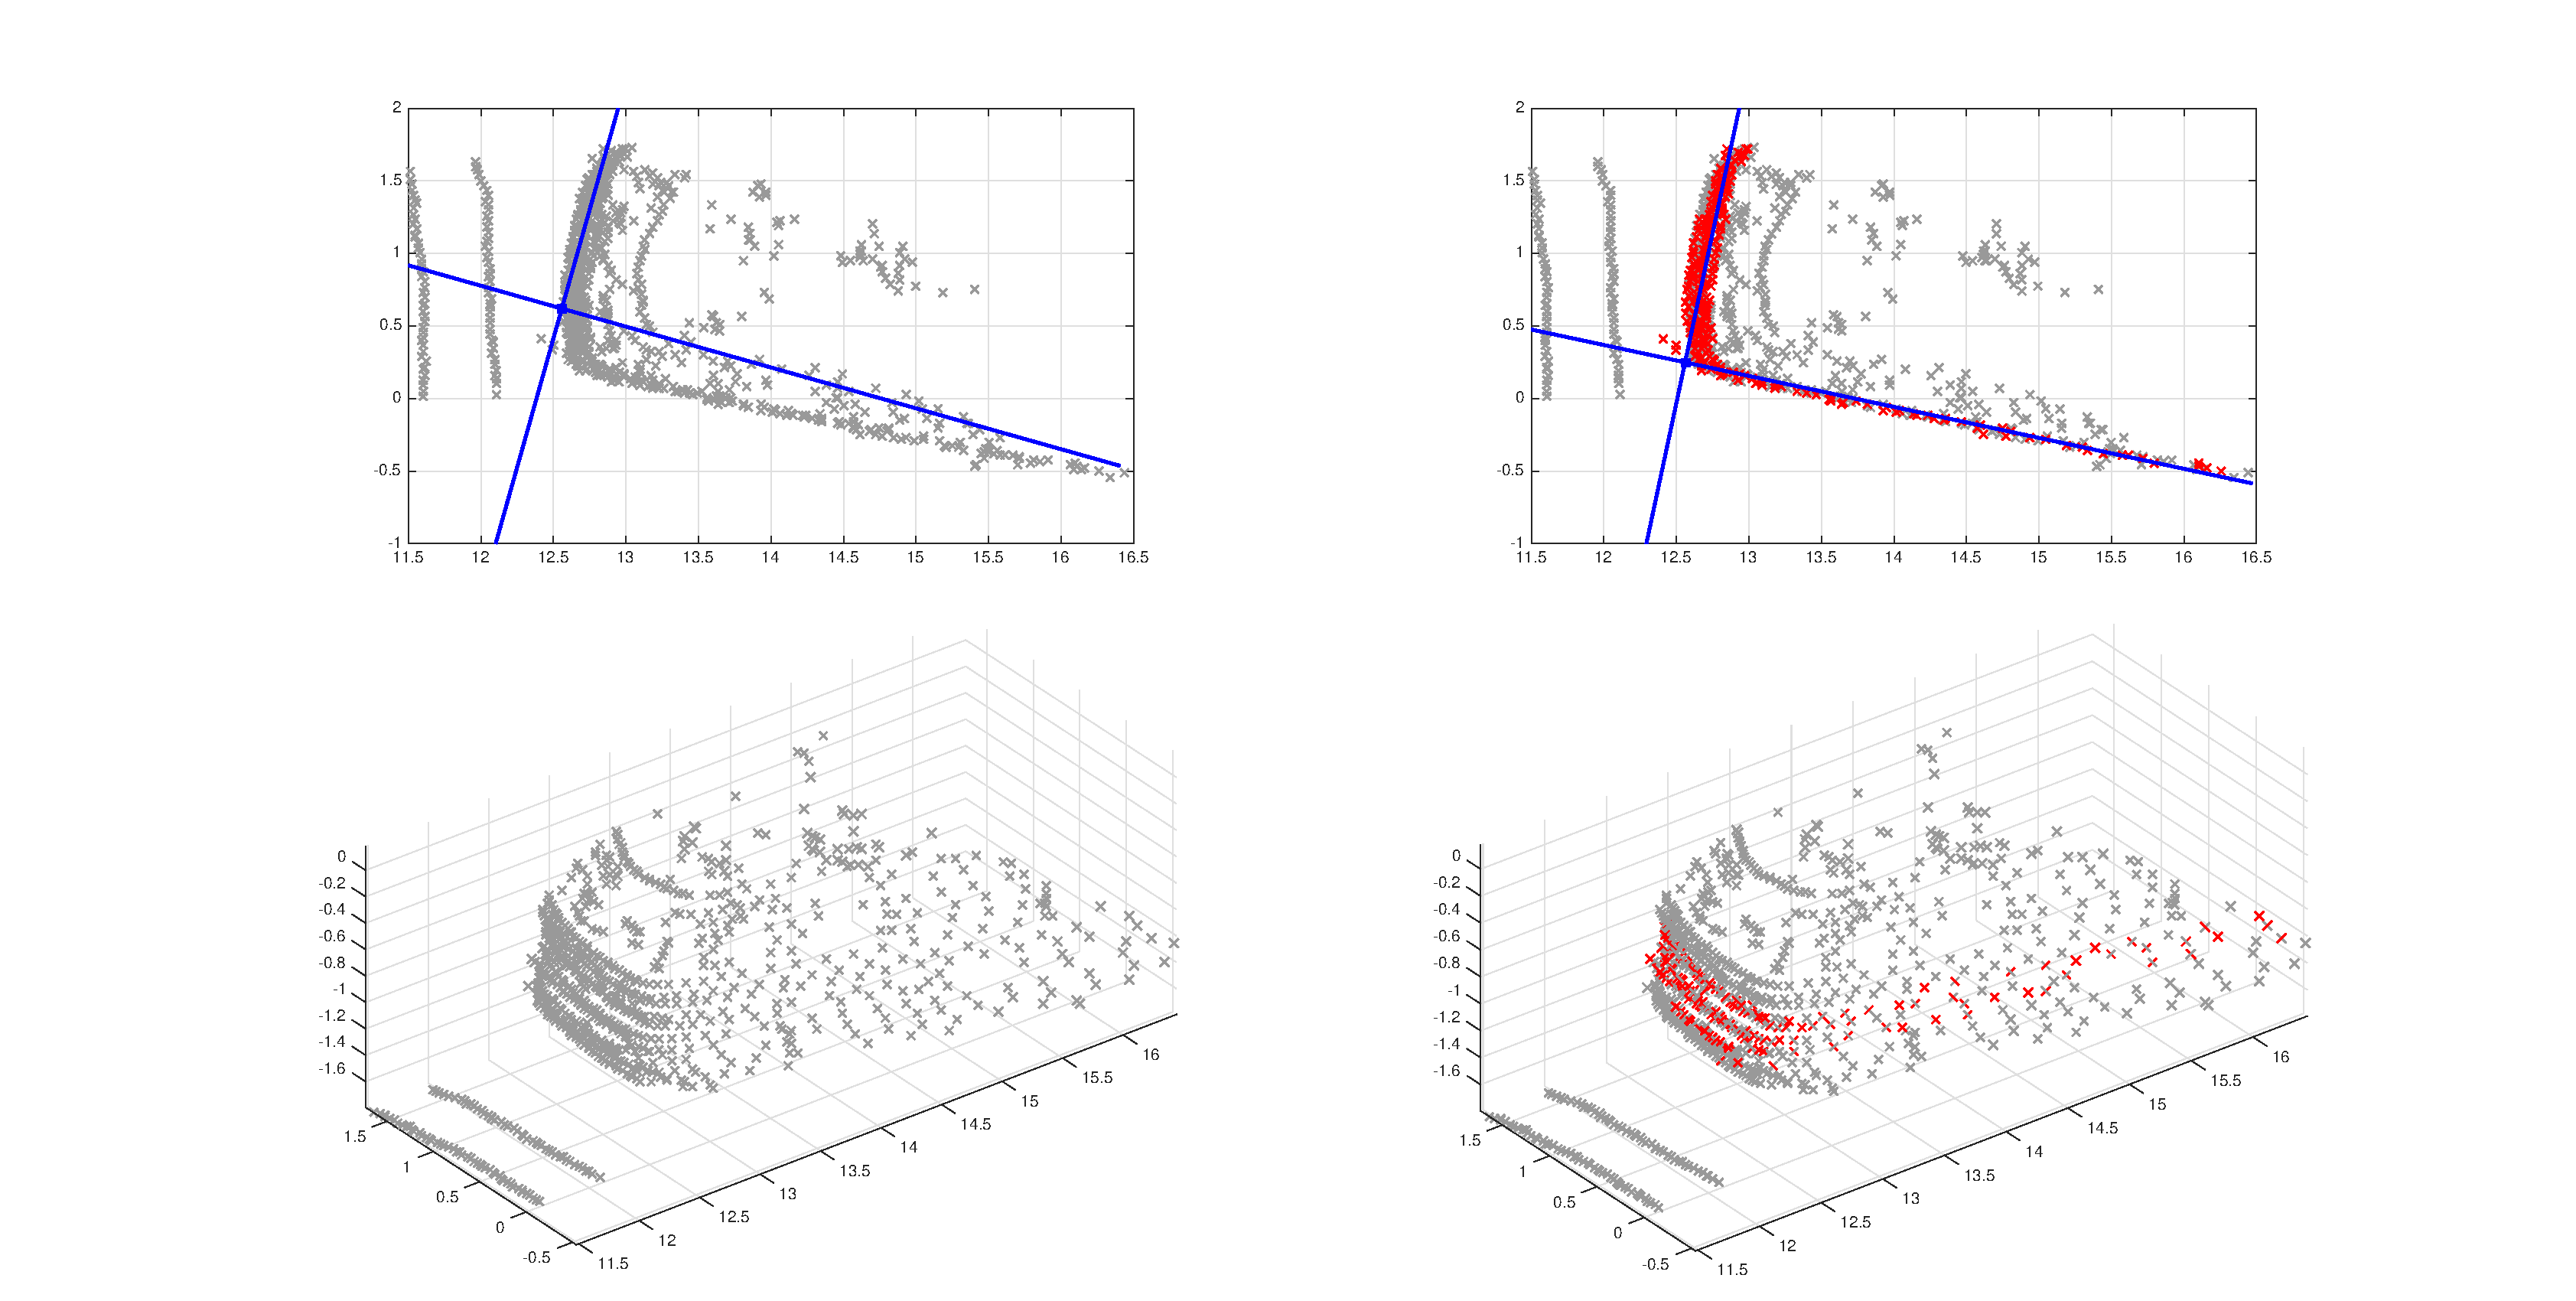
\includegraphics[width = \linewidth]{include/images/2by2.eps}
    \caption{This should be a 2x2 subplot, where to the left we see L-shape fitting on all points, and to the right we see L-shape fitting with the filtered points}
    \label{fig:exCar}
\end{figure}

With these properties in mind, the mean height $\mu_z$ of all measurements should be skewed towards measurement layers not encompassing any of the car's windows or curved surfaces. As such, measurements can first be filtered based on height, where measurements within in a bound around the mean height $\mu_z$ are kept.

The remaining measurements are then used in the ISED method. This will not only result in a more accurate estimate gained from ISED, but it also reduces computational complexity. Filtering lidar measurements based on height is a cheap operation since each lidar scan is ordered by height. Height filtering will also reduce the amount of measurements used in ISED, which also reduces computational complexity since less measurements need to be sorted according to bearing beforehand. Additionally, since computational complexity in ISED scales linearly with the amount of measurements, reducing the amount of measurements will also result in more efficient L-shape fitting. 

In this work the following bound was used for height-based filtering of car clusters measurements, where $\sigma_z$ is the standard deviation of the height of all measurements. The bound is skewed more towards lower layers since these layers encompass more surface area of the car, while measurements from layers above the mean risk encompassing windows and curved surfaces. This choice in parameters resulted on average in a $75\%$ decrease in the number of measurements used for L-shape fitting. 

\begin{equation}
     \mu_z - 0.50\sigma_z < z_k^i < \mu_z + 0.25\sigma_z
\end{equation}

\subsection{Supplementary Filtering}
While height based filtering works well for accurately fitting an L-shape to data, it does result in a significant loss of measurements. This can lead to informative measurements regarding the length of each side to be omitted, which is why supplementary filtering can used after height based filtering. Supplementary filtering utilizes the estimated corner point and orthogonal lines from ISED to essentially form a gate around the estimated L-shape. Supplementary filtering operates on \underline{all} measurements, which enables more accurate estimates of length and width. However, it also results in an increased amount of measurements for subsequent steps in the algorithm as compared to using measurements after height based filtering. The algorithm implemented in this work was tested both with and without use of supplementary filtering, see section XXX.
More detailed information regarding supplementary filtering can be found in Appendix XXX.

\subsection{Estimating length of viewed sides}

The corner point and orthogonal lines from ISED can be used in order to estimate the length of each viewed side. The remaining measurements from the filtering step are projected onto each of the orthogonal lines. The two largest distances between the corner point and a measurement from each set of projected measurements correspond to the viewed lengths. 

It is important to note that at this step in the algorithm it is not possible to distinguish between which side corresponds to a car's width or length, and by extension which corner of the car that is in view. This is dependent on the predicted car state, see section XXX for more information.

\subsection{Measurement Selection}
An important problem when tracking rectangular targets is how to assign measurements to each MGP. One solution to this problem, when dealing with radar measurements sorted by bearing, involves associating an MGP to each measurement present in the car cluster, see REF XXX. Such a solution has two general drawbacks when dealing with a lidar sensor. Firstly, the large amount of measurements per car will result in increased computational complexity. Secondly, such a solution is based on the assumption that measurements are uniformly distributed along each side of the car. This assumption does not hold when using lidar data, since other objects placed in between the lidar sensor and surrounding cars will result in regions of some cars being subject to occlusion, as in Figure \ref{fig:pocket}.

\begin{figure}[ht]
    \centering
    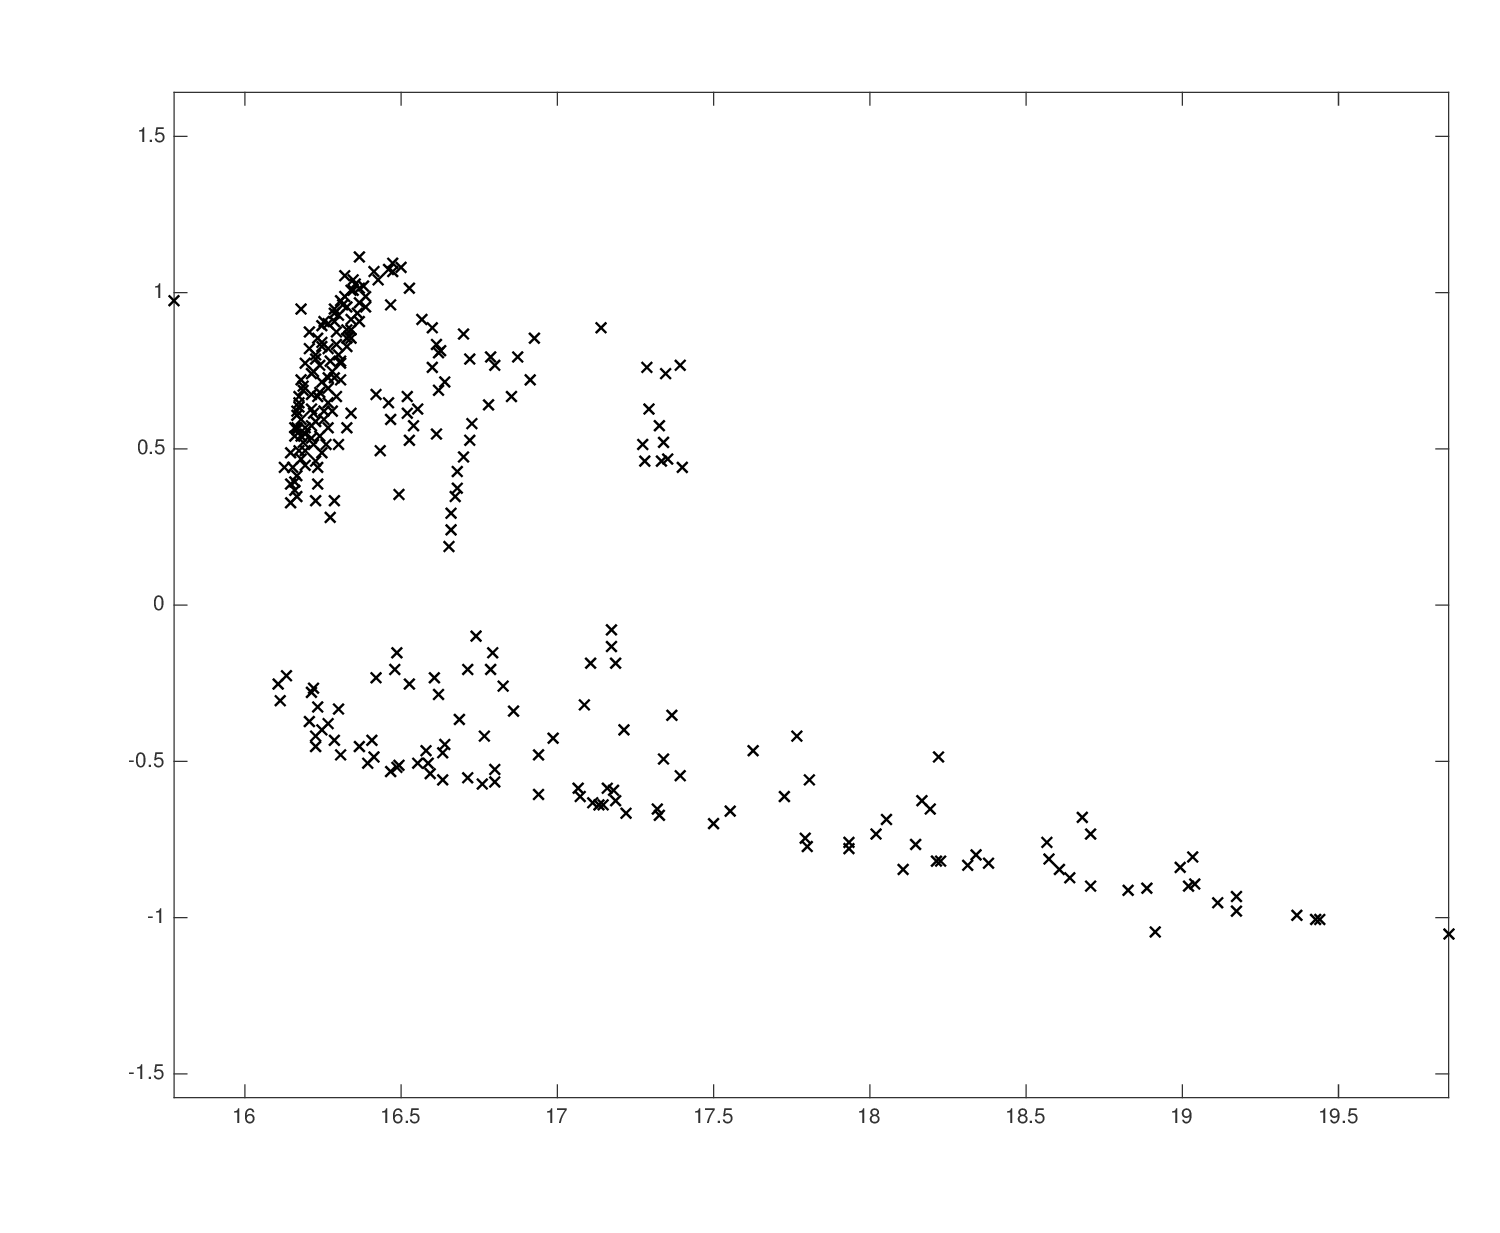
\includegraphics[width = 0.6\linewidth]{include/images/pocket.png}
    \caption{Caption}
    \label{fig:pocket}
\end{figure}

The solution to the measurement assignment problem in this work relies on the estimated corner point and orthogonal lines from the ISED method, while not suffering from the drawbacks listed above. By using the orthogonal lines attained from fitting an L-shape, a 2 dimensional vector $\mathbf{v}$ can be defined for each visible side (i.e. orthogonal line), where the magnitude of each vector is equal to the viewed length $\varepsilon$ of its corresponding side (calculated as per section XXX), see Figure \ref{fig:vectors}

\begin{align}
     \mathbf{v}_{1},\quad ||\mathbf{v}_{1}|| &= \varepsilon_{1} \\
     \mathbf{v}_{2},\quad ||\mathbf{v}_{2}|| &= \varepsilon_{2}
\end{align}

\begin{figure}[ht]
    \centering
    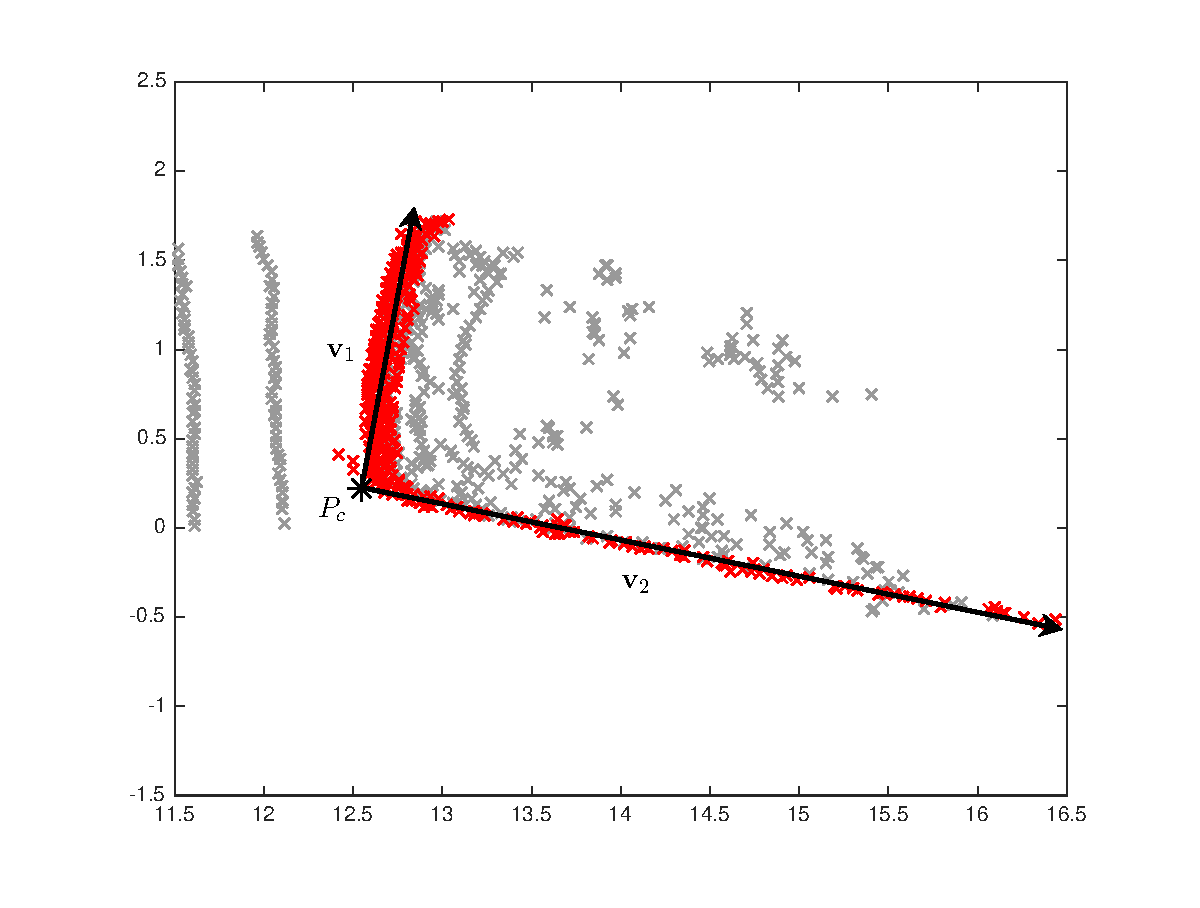
\includegraphics[width = 0.5\linewidth]{include/images/vectors.eps}
    \caption{Caption}
    \label{fig:vectors}
\end{figure}

These vectors can be used to create uniformly distributed \emph{ideal} MGPs $\delta_i$ along each visible side. The ideal MGPs $\delta_i$ represent positions along the car's length and width where we ideally would like place MGPs, since by definition a \emph{measurement generating point} is considered as a specific point which at each time step (potentially) generates a sensor measurement. By creating ideal MGPs and assigning them measurements, the same assignment can later be used when constructing MGPs based on the predicted state, $\mu_i(\xi_{k|k-1})$.\todo{I should explain this more.}

As such, under the presence of no occlusion, the ideal MGPs are uniformly distributed. Consequently, $1 + 2N$ ideal MGPs $\delta_i$ are created in the following way

\begin{align}
    \delta_0 &= P_c 
    \nonumber\\
    \delta_i &= G(P_c, i, N, \mathbf{v}_1) = P_c + \frac{i}{1+N}\mathbf{v}_1, & i = 1,2,\dots,N \\
    \delta_{i+N} &= G(P_c, i, N, \mathbf{v}_2) = P_c + \frac{i}{1+N}\mathbf{v}_2, & i = 1,2,\dots,N 
    \nonumber
\end{align}

where $P_c$ is the corner point, calculated with ISED. The resulting ideal MGPs are uniformly placed along the vectors $\mathbf{v}_1$ and $\mathbf{v}_2$. Each $\delta_i$ needs to be associated with a measurement, which can be performed by conducting a nearest neighbor search. Note that special care needs to be taken in order for no duplicate measurements to appear among assigned measurements; each measurement can by definition only be associated to one MGP. If the distance between an ideal MGP $\delta_i$ and its associated measurement $z_i$ is above the threshold $d_{max}$, then the ideal MGP is not assigned a measurement. Given how closely spaced lidar measurements are, the threshold $d_{max}$ will make sure that ideal MGPs placed in occluded regions are not included for later use in the car PHD filter. 

An additional threshold, $\varepsilon_{min}$, is used for determining whether one or both sides of the L-shape are visible enough to be used for state estimation. Consequently, if any of the vectors $\mathbf{v}_1$ and $\mathbf{v}_2$ has a magnitude less than $\varepsilon_{min}$ then no MGPs will be created for the associated side, resulting in a one-sided measurement update in Section XXX.

By formulating the two vectors $\mathbf{v}_1$ and $\mathbf{v}_2$, this method enables an upper limit of $N_{\lambda} = 1+2N$ measurements to be associated (and by extension the number of MGPs), thus making it possible to adjust computational complexity, although at the expense of state estimation accuracy. Additionally, the distance threshold $d_{max}$ can be used to take occluded regions into account. 


\begin{algorithm}[H]
\caption{Select Measurements}\label{meas}
\begin{algorithmic}
\Input $P_c$, $\mathbf{v}_1$, $\mathbf{v}_2$, $d_{max}$, $\varepsilon_{min}$, $N$, Set of measurements $Z$
%\Init Sort $C$ by distance to current ego position (ascending)
\State $\delta_0 = P_c$
\If{$||\mathbf{v}_1|| >\varepsilon_{min}$}
\For{$i = 1$ to $N$}
\State $\delta_i \leftarrow G(P_c, i, N, \mathbf{v}_1)$
\EndFor
\EndIf
\If{$||\mathbf{v}_2|| >\varepsilon_{min}$}
\For{$i = 1$ to $N$}
\State $\delta_{i+N} \leftarrow G(P_c, i, N, \mathbf{v}_1)$
\EndFor
\EndIf
\For{$j = 1$ to $|\delta|$}
\State $\{z_j,d_j\} \leftarrow$ unique nearest neighbor search for $\delta_j$
\If{$d_j > d_{max}$}
\State $z_j = \text{Null}$
\EndIf
\State $Z_a \leftarrow$ add $z_j$ to $Z_a$ 
\EndFor
\Output Vector of assigned measurements $Z_{a}$
\end{algorithmic}
\end{algorithm}

After conducting pre-processing for all car cluster measurements, each car cluster $C_{\text{car}}^{i}$ passed to the rectangular PHD filter will consist of the following set

\begin{equation}
    \begin{split}
        C_{\text{car}}^{i} &= \{Z^i_a, \mathbf{v}_{1}^i, \mathbf{v}_{2}^i\}
    \end{split}
\end{equation}

where $Z^i_a$ are the assigned measurements and $\mathbf{v}_{1}^i, \mathbf{v}_{2}^i$ are the vectors spanning each viewed side. 

\section{Rectangular PHD filter}

The rectangular PHD filter incorporates the general recursive equations presented in section XXX, with the main difference consisting of how each target is represented. In the general PHD recursion, each target consists of a single Gaussian component; this enables use of the basic KF equations found in section XYX to calculate all key steps during a PHD recursion: \textsc{Prediction}, \textsc{Likelihood} and \textsc{Update}. For rectangular tracking however, each component is instead represented by an IMM filter. In turn, the IMM filter utilizes either the EKF or UKF equations to perform necessary steps for each mode in the IMM filter. 

As such, motion models for use in the IMM filter need to be defined, as well as MGP-functions for each prediction, in order to perform all key steps in the PHD recursion. 


\subsection{Choice of Motion Models}
In this work, the IMM framework is used to incorporate two different motion models, one model for when the car is turning and one for when the car is driving straight. In order to incorporate both of these behaviours the following extended state vector is used

\begin{equation}
    \begin{split}
        \xi = [x\enspace y\enspace v\enspace \phi \enspace \dot{\phi} \enspace w \enspace l]^T
    \end{split}
\end{equation}

where $x$ and $y$ denote the mid-point of the car, $v$ is velocity, $\phi$ and $ \dot{\phi}$ are heading and turning-rate, $w$ and $l$ are the width and length on the car respectively. The two different motion models, $f^{t}(\xi)$ and $f^{s}(\xi)$, where $t$ denotes the model for turning, and $s$ denotes the model for driving straight, are defined in the following way, where $\Delta T = 0.1$sec is Lidar sample time.

\begin{equation}
    \begin{split}
        \xi_{k+1}^t
        = f^{t}(\xi_{k}) &= 
            \begin{bmatrix}
                x_k + \Delta T v_k\cos(\phi) \\
                y_k + \Delta T v_k\sin(\phi) \\
                [v_k, \enskip
                \phi_k + \Delta T \dot{\phi}_{k}, \enskip
                \dot{\phi}_{k}, \enskip
                w_k, \enskip
                l_k]^T
            \end{bmatrix} + q^t_k,
    \end{split}
\end{equation}
\begin{equation}
    \begin{split}
        \xi_{k+1}^s
        = f^{s}(\xi_{k}) &=
            \begin{bmatrix}
                x_k + \Delta T v_k\cos(\phi) \\
                y_k + \Delta T v_k\sin(\phi) \\
                [v_k, \enskip
                \phi_k, \enskip
                0, \enskip
                w_k, \enskip
                l_k]^T
            \end{bmatrix} + q^{s}_{k}
    \end{split}
\end{equation}

\begin{align}
        q_{k}^{t}
        \sim \mathcal{N}\left(\mathbf{0}_{7\times1}, Q_{t}\right), 
    &&   
        Q_{t} = \Gamma_t^T
        \begin{bmatrix}
            \sigma_v^2 & 0 & 0 & 0 \\ 
            0 & \sigma_{\dot{\phi}}^2 & 0 & 0 \\
            0 & 0 & \sigma_w^2 & 0 \\
            0 & 0 & 0 & \sigma_l^2
        \end{bmatrix}
        \Gamma_t,
    &&
        \Gamma_t = 
            \begin{bmatrix}
                0 & 0 & 1 & 0 & 0 & 0 & 0 \\
                0 & 0 & 0 & 0 & 1 & 0 & 0 \\
                0 & 0 & 0 & 0 & 0 & 1 & 0 \\
                0 & 0 & 0 & 0 & 0 & 0 & 1
            \end{bmatrix}
        \\  
        q_{k}^{s}
        \sim \mathcal{N}\left(\mathbf{0}_{7\times1}, Q_{s}\right), 
    &&   
        \Sigma_s = \Gamma_s^T
        \begin{bmatrix}
            \sigma_v^2 & 0 & 0 & 0 \\
            0 & \sigma_{\phi}^2 & 0 & 0 \\
            0 & 0 & \sigma_w^2 & 0 \\
            0 & 0 & 0 & \sigma_l^2 
        \end{bmatrix}
        \Gamma_s,
    && 
        \Gamma_s = 
            \begin{bmatrix}
                0 & 0 & 1 & 0 & 0 & 0 & 0 \\
                0 & 0 & 0 & 1 & 0 & 0 & 0 \\
                0 & 0 & 0 & 0 & 0 & 1 & 0 \\
                0 & 0 & 0 & 0 & 0 & 0 & 1
            \end{bmatrix}
\end{align}

With the two motion models defined, calculating each prediction $\xi_{k|k-1}^t, \xi_{k|k-1}^s$ is performed by

\begin{equation}
    \begin{split}
    \{\hat{\xi}^{0t}_{k|k-1}, P_{k|k-1}^{0t}, \hat{\xi}^{0s}_{k|k-1}, P_{k|k-1}^{0s}\} &= \textsc{IMM.Mixing}\left(\hat{\xi}^{t}_{k-1|k-1}, P^{t}_{k-1|k-1},\hat{\xi}^{s}_{k-1|k-1}, P^{s}_{k-1|k-1}\right)
    \\
        \{\hat{\xi}^t_{k|k-1}, P_{k|k-1}^t\} &= \textsc{IMM}.\textsc{Predict}\left(f^t(\cdot),\enskip \hat{\xi}^{0t}_{k|k-1}, P_{k|k-1}^{0t}\right)
    \\
        \{\hat{\xi}^s_{k|k-1}, P_{k|k-1}^s\} &= \textsc{IMM}.\textsc{Predict}\left(f^s(\cdot),\enskip \hat{\xi}^{0s}_{k|k-1}, P_{k|k-1}^{0s}\right)
    \end{split}
\end{equation}

The \textsc{IMM} block first performs \todo{REF}mixing in order to get mixed estimates, before the \textsc{Predict} operation is called, which can either be performed using the EKF predict or UKF predict\todo{ref} equations. 

\subsection{Generating Measurement Generating Points}

In order to calculate the likelihood and update for each estimate, MGPs need to be created for each prediction. From the pre-processing step, each car cluster $C_{\text{car}}^{i}$ consists of 

\begin{equation}
    \begin{split}
        C_{\text{car}}^{i} &= \{Z^i_a, \mathbf{v}_{1}^i, \mathbf{v}_{2}^i\}
    \end{split}
\end{equation}

where $Z^i_a$ are the assigned measurements and $\mathbf{v}_{1}^i, \mathbf{v}_{2}^i$ are the vectors spanning each viewed side. As such, in order to generate MGPs the vectors $\mathbf{v}_{1}^i, \mathbf{v}_{2}^i$ must be identified by which side they correspond to (i.e. which vector is width and which is length), and by extension from which corner point $P_c$ they originate from (i.e. $P_c$ corresponds to either corner $1,2,3,4$). This is important, since selection and ordering of the assigned measurements $Z_a$ is dependent on the viewed corner in the pre-processing step.

The implication of this is that each prediction will act as a form of hypothesis regarding which corner (and by extension which sides) are seen in the data. This results in MGPs-generation which is dependant on predicted state. This can most easily be illustrated by viewing Figure \ref{fig:diffPred}.

\begin{figure}[ht]
    \centering
    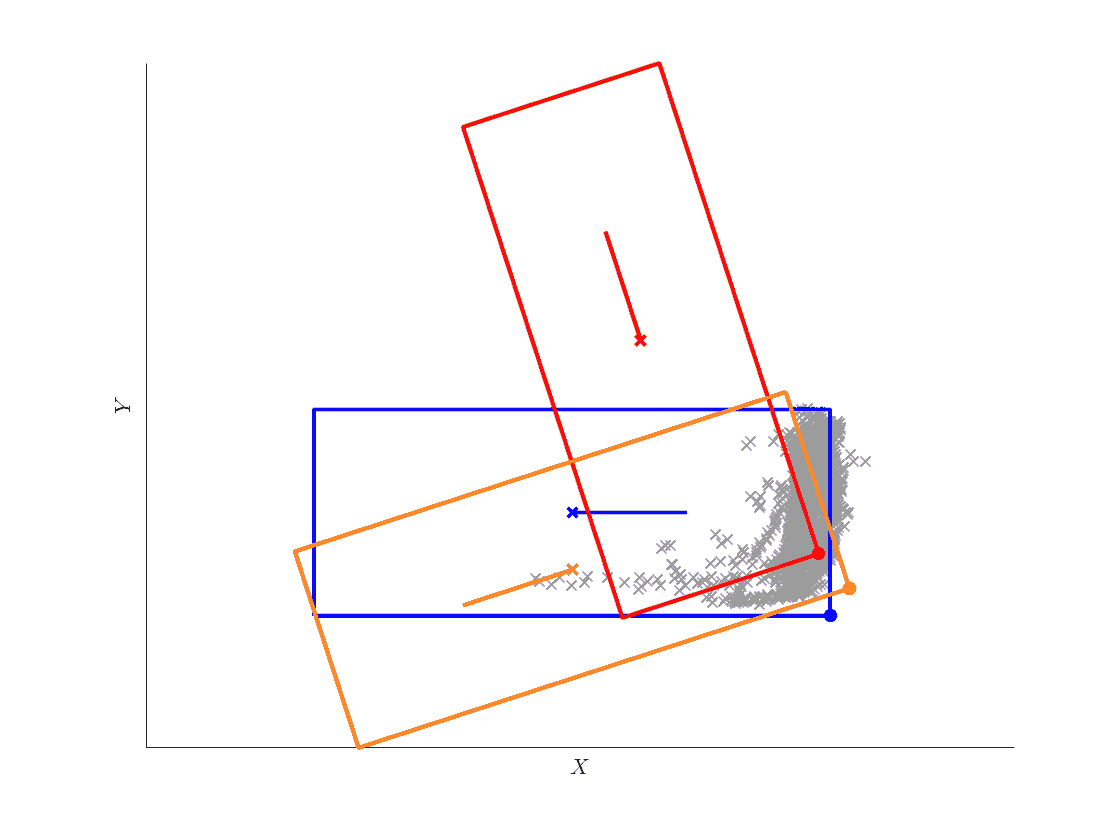
\includegraphics[width = 0.5\linewidth]{include/images/diffPred.png}
    \caption{This figure lacks a lot of things}
    \label{fig:diffPred}
\end{figure}

In the figure all measurements constituting the car cluster are seen, as well as predictions from three different IMM components, each with a different color. Since each IMM component consists of the two motion models defined in section XXX, two predictions exist for each component, distinguished with solid and dashed lines. 

The two vectors $\mathbf{v}_{1}^i, \mathbf{v}_{2}^i$ are known since pre-processing has occurred, and as such a number of assigned measurements have already been chosen. In the figure a total of XX measurements have been chosen. Since there exists ambiguity in which corner of the car is actually seen, each IMM component will act as a hypothesis on this matter. In the case of the red component, the corner point is seen as $P_c \rightarrow \text{corner}_1$ according to our definition (See Section XXX). For the blue and orange components, the corner will be seen as $P_c \rightarrow \text{corner}_4$ and $P_c \rightarrow \text{corner}_2$ respectively. Depending on how the car behaves in the next time step, only one (or none) of these three components will prove to be correct. As such, if one of these predictions proves to be valid, it will result in a higher weight for said component in the PHD filter.

The choice in which corner is seen is solely dependant on predicted heading $\phi_{k|k-1}$, and can be determined by utilizing linear algebra. Consequently, deciding which side the vectors $\mathbf{v}_{1}^i, \mathbf{v}_{2}^i$ belong to is also dependant on predicted heading and can also be determined with linear algebra. Knowledge about corner point and which side is seen, are necessary to construct MGPS for each prediction. The necessary steps for deciding corner and which sides are seen can be found in Algorithm \ref{cp} and \ref{len}.


\begin{algorithm}[H]
\caption{Identify which corner is seen}\label{cp}
\begin{algorithmic}
\Input $\phi_{k|k-1}$, $\mathbf{v}_1$, $\mathbf{v}_2$
\Init{Generate unit vectors of $\mathbf{v}_1$, $\mathbf{v}_2$: $\mathbf{u}_1$, $\mathbf{u}_2$}
\State \textit{Inverse rotate each unit vector with the predicted heading}
\State $\mathbf{u}_1^{0}  \leftarrow \text{inv.rot}(\mathbf{u}_1, \phi_{k|k-1})$
\State $\mathbf{u}_2^{0}  \leftarrow \text{inv.rot}(\mathbf{u}_2, \phi_{k|k-1})$
\State \textit{Calculate angle $0 \leq \psi \leq 2\pi$}
\State $\psi \leftarrow \arccos(\text{dot}(\mathbf{u}_1^{0},\mathbf{u}_2^{0}))$, 
\If{$0<\psi\leq \pi/2$}
\State corner $= 1$
\ElsIf{$\pi/2<\psi\leq \pi$}
\State corner $= 4$
\ElsIf{$\pi<\psi\leq 3\pi/2$}
\State corner $= 3$
\ElsIf{$3\pi/2<\psi\leq 2\pi$}
\State corner $= 2$
\EndIf
\Output{corner}
\end{algorithmic}
\end{algorithm}

\begin{algorithm}[H]
\caption{Identify viewed width and length}\label{len}
\begin{algorithmic}
\Input $\phi_{k|k-1}$, $\mathbf{v}_1$, $\mathbf{v}_2$
\Init{Generate unit vectors of $\mathbf{v}_1$, $\mathbf{v}_2$: $\mathbf{u}_1$, $\mathbf{u}_2$}
\State \textit{Construct unit vector representing $\phi_{k|k-1}$}
\State $\mathbf{u}_{\phi} = [\cos(\phi), \sin(\phi)]^T$
\If{$\text{dot}(\mathbf{u}_{\phi}, \mathbf{u}_{1}) > \text{dot}(\mathbf{u}_{\phi}, \mathbf{u}_{2})$}
\State $s_1 = "\text{length}"$
\State $s_2 = "\text{width}"$
\State $l_{view} = ||\mathbf{v}_1||$
\State $w_{view} = ||\mathbf{v}_2||$
\Else
\State $s_1 = "\text{width}"$
\State $s_2 = "\text{length}"$
\State $w_{view} = ||\mathbf{v}_1||$
\State $l_{view} = ||\mathbf{v}_2||$
\EndIf
\Output{$s_1, s_2, w_{view}, l_{view}$}
\end{algorithmic}
\end{algorithm}

After performing the steps detailed in Algorithm \ref{cp} and \ref{len}, MGP functions can be generated for each prediction and associated measurement. It is important to note that we are \underline{not creating MGPs}, instead we are creating MGP-\textit{functions}. Revisiting the general MGP equations from Section XXX, 

\begin{align}
    \{h_{l}^j(\xi_{\text{\tiny{min}}})\}_{j = 1}^{N} &= h_c^i(\xi_{\text{\tiny{min}}}) + \frac{j}{1+N}\rho_l
        \begin{bmatrix}
            l\cos(\phi + \eta(i)) \\
            l\sin(\phi + \eta(i)) 
        \end{bmatrix}, & \eta(i) &\rightarrow \{0,0,\pi,\pi\} 
    \\\nonumber 
    \\ 
    \{h_{w}^j(\xi_{\text{\tiny{min}}})\}_{j = 1}^{N} &= h_c^i(\xi_{\text{\tiny{min}}}) + \frac{j}{1+N}\rho_w
    \begin{bmatrix}
        w\cos(\phi + \eta(i)) \\
        w\sin(\phi + \eta(i)) 
    \end{bmatrix}, & \eta(i) &\rightarrow \left\{\frac{\pi}{2},\frac{3\pi}{2},\frac{3\pi}{2},\frac{\pi}{2}\right\} 
\end{align}

we can see that while they do depend on the state $\xi$, they also depend on a number of other variables as well: $i$, $N$, $\rho_w$ and $\rho_l$. The variable $i$ represents the corner point, which at this point is determined with Algorithm \ref{cp}. The variable $N$ represents the number of MGPs, which is also known since $1 + 2N$ measurements are assigned at the pre-processing step (the parameter $N$ is user selected). The two ratios, $\rho_l$ and $\rho_w$ are also known, since both predicted state $\xi_{k|k-1}$ as well as $w_{view}$ and $l_{view}$ are known (Algorithm \ref{len}). As such, constructing a vector of MGP-functions corresponds to using the general equations together with the state-independent parameters ($i$, $N$, $\rho_w$ and $\rho_l$) to form MGP-functions which solely depend on the state $\xi$. Since assigned measurements $Z_a^i$ are ordered according to $P_c$-MGP, $\mathbf{v}_1$-MGPs and $\mathbf{v}_2$-MGPs, the MGP-functions need to be generated in same order. The same threshold for viewed length and width, $\varepsilon_{min}$, is also used when generating MGP-functions. 

For example, for $N = 2$, $corner = 1$, $\rho_w = \rho_l = 1$, $\varepsilon_1 > \varepsilon_{min}$, $\varepsilon_2 > \varepsilon_{min}$ and where $\mathbf{v}_1$ corresponds to width, the MGP-function vector is the following:

\begin{equation}
    \begin{split}
        H(\xi) &= 
        \underbrace{\begin{bmatrix}
            h_c^{i=1}(\xi) \\
            h_w^{1}(\xi, \rho_w = 1, i=1) \\
            h_w^{2}(\xi, \rho_w = 1, i=1) \\
            h_l^{1}(\xi, \rho_l = 1, i=1) \\
            h_l^{2}(\xi, \rho_l = 1, i=1)
        \end{bmatrix}}_{\mathbf{2(1+4)\times1}}
    \end{split}
\end{equation}

The final step, before using the $H(\xi)$ function vector and the assigned measurements $Z_a^i$ for \textsc{Update} or \textsc{Likelihood}, is to remove empty measurements from $Z_a^i$ and their corresponding MGP-functions from $H(\xi)$. This is since empty measurements fall outside of the threshold $d_{max}$, indicating that an occluded region is present for the corresponding MGP-functions. 

\subsection{Incorporating Rectangular Targets in PHD recursion}

With motion models defined, as well as the capability to generate MGP-functions for each prediction in an IMM component, an entire PHD recursion can be computed. The prerequisites 

\begin{algorithm}[H]
\caption{A single PHD recursion for Rectangular Targets. NEEDS MORE WORK}\label{rectPHD}
\begin{algorithmic}
\Input 
Number of components to keep between recursions $N_{\text{\tiny{PHD}}}$, 
Survival prob $P_s$, 
Detection prob $P_D$,
Birth PHD $\gamma_k(\xi)$,
Previous PHD $v_{k-1}(\xi)$,
Clutter Rate $K$,
Individual MGP covariance $\sigma_R^2$,
Max number of MGPs per side $N$,
MGP to measurement distance threshold $d_{max}$,
Viewed side threshold $\varepsilon_{min}$,
Measurement clusters $\{C^i_{\text{car}}=\{Z_a^i,\mathbf{v}_1,\mathbf{v}_1\}\}_{i=1}^m$
\State 
\State \textit{Perform prediction on previous set}
\State $v_{k|k-1} \leftarrow \gamma_k(\xi)$
\For{$j = 1,\dots,N_{\text{\tiny{PHD}}}$}
\State \textit{Predict each IMM component in previous PHD $v_{k-1}(\xi)$}
\State $v_{k|k-1} \leftarrow \textsc{IMM}(j)\textsc{.Predict}$
\EndFor
\State \textit{Calculate updated PHD}
\State $v_{k|k}(\xi) \leftarrow (1-P_D)v_{k|k-1}(\xi)$
\For{$i = 1, \dots, m$}
\For{$j = 1, \dots, N_{\text{\tiny{PHD}}}$}
\State Algorithm 5
\State Algorithm 6
\State $H(\xi)\leftarrow$ Algorithm XYX
\State $w_{k|k}^j\leftarrow P_D\times w_{k|k-1}^j\times$\textsc{IMM.Likelihood}$(Z_a^i, H(\xi),\sigma_R^2)$
\EndFor
\For{$j = 1, \dots, N_{\text{\tiny{PHD}}}$}
\State $w_{k|k}^j\leftarrow$ Normalize with $K +\sum_{j=1}^{N_{\text{\tiny{PHD}}}}w_{k|k-1}^j$
\EndFor
\EndFor
\Output{$s_1, s_2, w_{view}, l_{view}$}
\end{algorithmic}
\end{algorithm}


















